%You can leave alone everything before Line 79.
\documentclass{article}
\usepackage{url,amsfonts, amsmath, amssymb, amsthm,color, enumerate, verbatim}
% Page layout
\setlength{\textheight}{8.75in}
\setlength{\columnsep}{2.0pc}
\setlength{\textwidth}{6.5in}
\setlength{\topmargin}{0in}
\setlength{\headheight}{0.0in}
\setlength{\headsep}{0.0in}
\setlength{\oddsidemargin}{0in}
\setlength{\evensidemargin}{0in}
\setlength{\parindent}{1pc}
\newcommand{\shortbar}{\begin{center}\rule{5ex}{0.1pt}\end{center}}
%\renewcommand{\baselinestretch}{1.1}
% Macros for course info
\newcommand{\courseNumber}{ME 552}
\newcommand{\courseTitle}{Mechatronics}
\newcommand{\semester}{Fall 2012}
\newcommand{\xxx}[1]{\textcolor{red}{#1}}
% Theorem-like structures are numbered within SECTION units
\theoremstyle{plain}
\newtheorem{theorem}{Theorem}[section]
\newtheorem{lemma}[theorem]{Lemma}
\newtheorem{corollary}[theorem]{Corollary}
\newtheorem{proposition}[theorem]{Proposition}
\newtheorem{statement}[theorem]{Statement}
\newtheorem{conjecture}[theorem]{Conjecture}
\newtheorem{fact}{Fact}
%definition style
\theoremstyle{definition}
\newtheorem{definition}[theorem]{Definition}
\newtheorem{example}{Example}
\newtheorem{problem}[theorem]{Problem}
\newtheorem{exercise}{Exercise}
\newtheorem{algorithm}{Algorithm}
%remark style
\theoremstyle{remark}
\newtheorem{remark}[theorem]{Remark}
\newtheorem{reduction}[theorem]{Reduction}
%\newtheorem{question}[theorem]{Question}
\newtheorem{question}{Question}
%\newtheorem{claim}[theorem]{Claim}
%
% Proof-making commands and environments
\newcommand{\beginproof}{\medskip\noindent{\bf Proof.~}}
\newcommand{\beginproofof}[1]{\medskip\noindent{\bf Proof of #1.~}}
\newcommand{\finishproof}{\hspace{0.2ex}\rule{1ex}{1ex}}
\def\therefore{\boldsymbol{\text{ }
\leavevmode
\lower0.4ex\hbox{$\cdot$}
\kern-.5em\raise0.7ex\hbox{$\cdot$}
\kern-0.55em\lower0.4ex\hbox{$\cdot$}
\thinspace\text{ }}}

\newenvironment{solution}[1]{\medskip\noindent{\bf Problem #1.~}}{\shortbar}

%====header======
\newcommand{\solutions}[4]{
%\renewcommand{\thetheorem}{{#2}.\arabic{theorem}}
\vspace{-2ex}
\begin{center}
{\small  \courseNumber, \courseTitle
\hfill {\Large \bf {#1} }\\
\semester, University of Michigan, Ann Arbor \hfill
{\em Date: #3}}\\
\vspace{-1ex}
\hrulefill\\
\vspace{4ex}
{\LARGE Lab Assignment #2}\\
\vspace{2ex}
\end{center}
\begin{trivlist}
\item \textsc{Team members:\\} {#4}
\end{trivlist}
\noindent
\shortbar
\vspace{3ex}
}
% math macros
\newcommand{\defeq}{\stackrel{\textrm{def}}{=}}
\newcommand{\Prob}{\textrm{Prob}}
\newcommand{\Lagr}{\mathcal{L}}
%==
\usepackage{graphicx}
\usepackage{xfrac}
\usepackage{amsmath}
\providecommand{\e}[1]{\ensuremath{\times 10^{#1}}}
\begin{document}
%%%%%%%%%%%%%%%%%%%%%%%%%%%%%%%%%%%%%%%%%%%%%%%%%
%\solutions{Your name}{Problem Set Number}{Date of preparation}{Collaborators}{Prover}{Verifiers}
\solutions{}{5: Stepper Motor}{\today}{Shiva Ghose, @gshiva\\ John Peterson, @jrpeters\\ Peter Turpel, @pturpel\\ Chan-Rong Lin, @pmelin}
%%%%%%%%%%%%%%%%%%%%%%%%%%%%%%%%%%%%%%%%%%%%%%%%%
%\renewcommand{\theproblem}{\arabic{problem}} 
%%%%%%%%%%%%%%%%%%%%%%%%%%%%%%%%%%%%%%%%%%%%%%%%%
%
% Begin the solution for each problem by
% \begin{solution}{Problem Number} and ends it with \end{solution}
%
% the solution for Problem 
\section*{Teamwork Participation Pledge :: Team 1}

I attest that I have made a fair and equitable contribution to this lab and submitted 
assignment. \\

My signature also indicates that I have followed the University of Michigan Honor Code, 
while working on this lab and assignment.\\

I accept my responsibility to look after all of the equipment assigned to me and my team, 
and that I have read and understood the X50 Lab Rules.\\

\begin{table}[h]
\begin{center}
    \begin{tabular}{|c|c|c|}
        \hline
        \textbf{Name} & \textbf{Email}     & \textbf{ \ \ \ \ \  \ \  \ \ \ \ \  \ \ Signature  \ \ \ \ \  \ \ \ \ \ \ \  \ \ } \\ \hline
        	~& ~& ~\\
	~& ~& ~\\
	Shiva Ghose   & gshiva@umich.edu   & ~                  \\
	~& ~& ~\\
	~& ~& ~\\ \hline 
	~& ~& ~\\
	~& ~& ~\\
        John Peterson & jrpeters@umich.edu & ~                  \\ 
	~& ~& ~\\
	~& ~& ~\\ \hline 
	~& ~& ~\\
	~& ~& ~\\
        Peter Turpel   & pturpel@umich.edu & ~                  \\
	~& ~& ~\\
	~& ~& ~\\ \hline 
	~& ~& ~\\
	~& ~& ~\\
        Chan-Rong Lin   & pmelin@umich.edu & ~                  \\
	~& ~& ~\\
	~& ~& ~\\ \hline 
        \hline
    \end{tabular}
\end{center}
\end{table}

\newpage

\section{Stepper Motor Driver}
\subsection*{a.}

\begin{figure}[htb]
\begin{center}
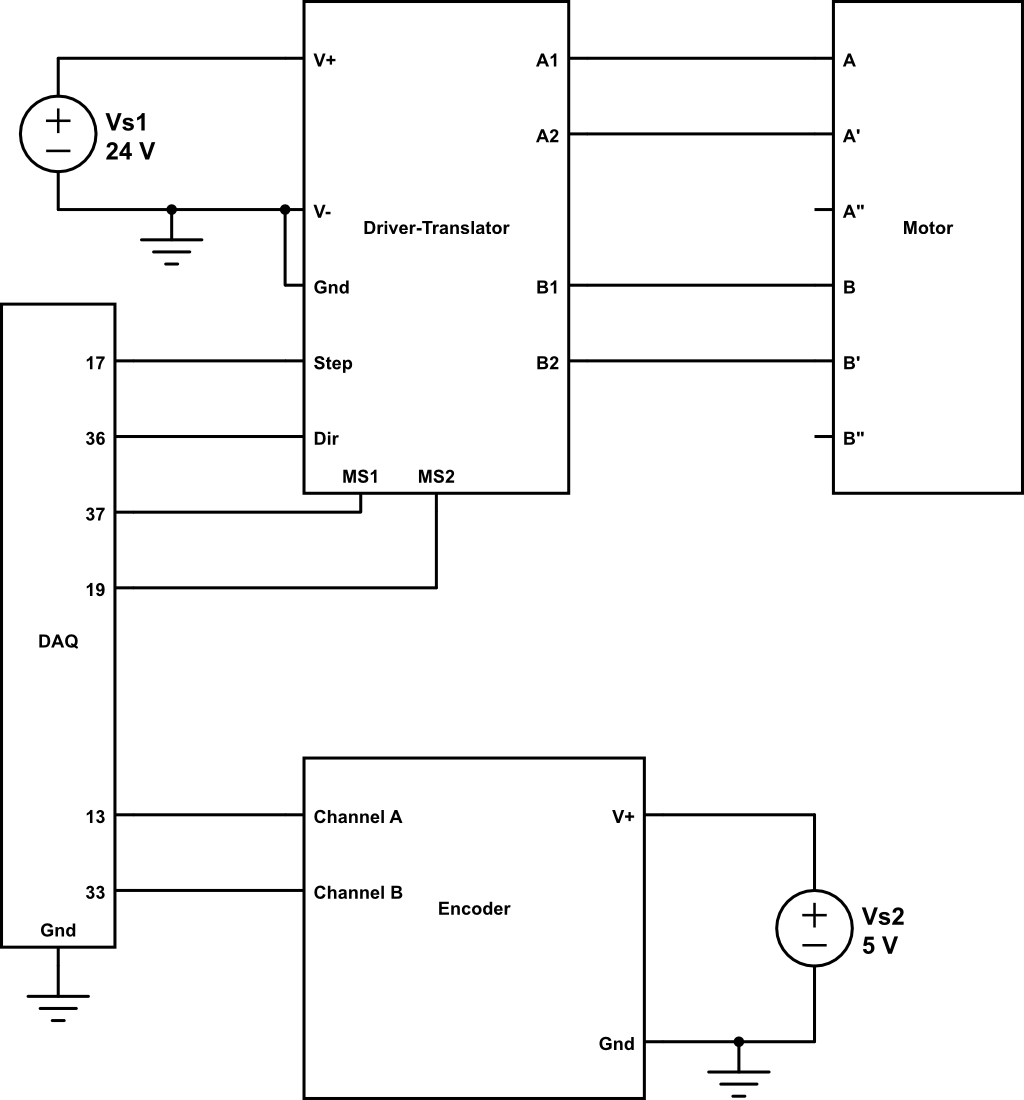
\includegraphics[width = 12cm]{lab5_main.png}
\caption{System level connection diagram. \xxx{Note all grounds are common}}
\label{q1_a}
\end{center}
\end{figure}

\subsection*{b.}
\begin{figure}[htb]
\begin{center}
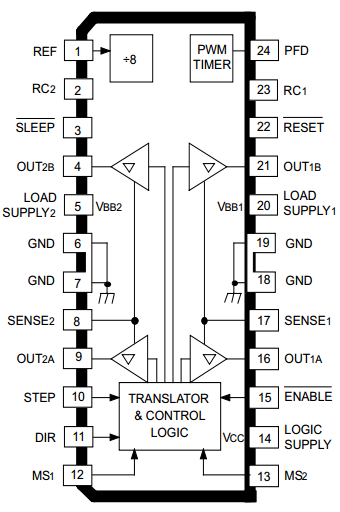
\includegraphics[width = 5cm]{A3967_pinout.png}
\caption{Pinout diagram of the A3967 chip.}
\label{q1_b}
\end{center}
\end{figure}

\begin{figure}[htb]
\begin{center}
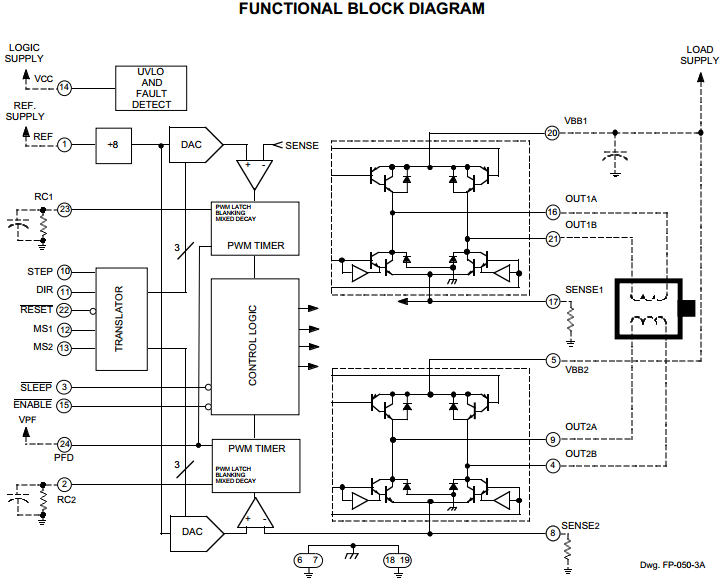
\includegraphics[width = 14cm]{A3967_functionalDiagram.png}
\caption{Functional diagram of the A3967 chip.}
\label{q1_b2}
\end{center}
\end{figure}

\subsubsection*{Pin1 - REF}
The \emph{REF} pin of the A3967 chip takes set the reference voltage for the logic circuit $V_{REF}$. It works with tandem with the senseristor to control the magnitude of the H-bridge current in the following manner:
\begin{itemize}
\item At $V_{REF} = 5$V max current will be 833mA.
\item At $V_{REF} = 3.3$V max current will be 550mA.
\item At $V_{REF} = 1$V max current will be 166mA.
\end{itemize}

From the functional diagram (figure \ref{q1_b2}), we see that $V_{REF}$ is fed into a DAC which is then fed to a comparator which then controls the PWM output, which in turn controls the current.\\

This input does not strictly require a dedicated external circuit, but the EasyDriver does provide a voltage divider circuit which is adjustable using a potentiometer thereby allowing us to \emph{tune} $V_{REF}$. 

\subsubsection*{Pin2 - RC2, Pin23 - RC1}
RC1 and RC2 control the fixed off-time for bridge 1 and bridge 2 respectively. Fixed off-time current regulation sets the current-decay modes of the H-bridges (slow, fast, or mixed).  The \emph{correct} current-decay control scheme can result in reduced audible motor noise, increased step accuracy, and reduced power dissipation.\\

According to the data sheet, the internal PWM current-control circuitry uses a one shot control scheme to regulate the time that the driver remains off.  The one shot off-time, $t_{off}$ , is determined by the selection of an external resistor ($R_T$) and capacitor($C_T$) connected from the $RC$ timing terminal to the ground. The off-time, over a range of values of $C_T = 470 pF$ to $1500 pF$ and $R_T = 12 k\Omega$ to $100 k\Omega$ is approximated by:
$$t_{off} = R_T C_T$$

The EasyDriver uses $R_T = 20k\Omega$ and $C_T = 680 pF$, hence $t_{off} = 0.0000136$s.\\

\subsubsection*{Pin3 - SLEEP}
This terminal allows us to minimize power consumption when not in use. It works by disabling most of the internal circuitry and switching of the outputs of the chip. It is an active-low terminla, meaning that for normal operation a 1-logic command/high voltage signal needs to be sent to it, while in order to set the system to sleep, a 0-logic command/low voltage signal needs to be sent instead. When starting up from a sleep command, the device will return to its default/home position.\\

The EasyDriver provides a pull up resistor in series with this terminal to ensure it doesn't load the circuit it is connected to and also to prevent currents from flowing through it.


\subsubsection*{Pin4 - OUT2B, Pin9 - OUT2A, Pin16 - OUT1A, Pin21 - OUT1B}
These pins are the outputs of the H-bridge. As seen in the functional bloack diagram (figure \ref{q1_b2}), OUT-\emph{x}-A and OUT-\emph{x}-B represent the outputs of H-bridge \emph{x} and together complete the circuit of the respective phase of the motor.\\

The EasyDriver provides pin-outs for these terminals through jumper 3 (JP3).

\subsubsection*{Pin5 - LOAD SUPPLY2, Pin17 - LOAD SUPPLY1}
These pins provide the input power for the H-bridge to supply the motors. The data-sheet of the A3967 chip suggests that the supply voltage should be decoupled with an electrolytic capacitor ($>$47 $\mu$F is recommended). This decoupling is not provided in the EasyDriver PCB.\\

The decoupling capacitors would provide isolation from the supply sources noise as well as provide temporary boosting-effects if the load changes suddenly. The EasyDriver circuit assumes that the supply-source can react instantaneously and is relatively noise free.
\xxx{PHYSICAL EXTRA IMPLEMENTATION}

\subsubsection*{Pin6 - GND, Pin7 - GND, Pin18 - GND, Pin19 - GND}
Connects various elements of the chip to the ground. The EasyDriver circuit takes care of this internally.

\subsubsection*{Pin8 - SENSE2, Pin17 - SENSE1}
The sense-terminals are connected to senseristors which measure the current flowing across them in order to control the output of the H-bridge. It forms a feed-back loop by acting as a \emph{sensor}. The EasyDriver PCB has 2 external sense-resistors of $0.75\Omega$, one for each H-bridge.

\subsubsection*{Pin10 - STEP}
The Step-terminal is an edge detector that operates on negative-positive changes in logic. On detecting such a transition, the  translator is told to advance the motor by one increment. Note that the input to the DACs and the direction of rotation are controlled by the translator itself, while the size of the increment is determined by the state of MS1  and MS2.\\

The EasyDriver provides direct access to this terminal through jumper 2 (JP2) and no external circuitry is required. A pull up resistor could be used just to be safe though.

\subsubsection*{Pin11 - DIR}
This pin determines the direction of rotation of the motor. The physical wiring of the motor decides which way the motor will actually rotate, however knowing that, this pin lets the user switch the direction digitally. The EasyDriver pcb allows for direct access of this pin through jumper 2 (JP2). Like the step control pin, a  pull up resistor could be used just to be safe.

\subsubsection*{Pin12 - MS1, Pin13 - MS2}





\subsubsection*{Pin24 - \xxx{PFD}}
When an input signal commands lowers the output current from the previous step, it switches the output current decay to either slow-, fast-, or mixed-decay depending on the voltage level at the RC terminal.  If the voltage is greater than 0.6$V_{CC}$ then slow-decay mode is selected.  If the voltage is less than 0.21$V_{CC}$ then fast-decay mode is selected.  Mixed decay is between these two levels and works by initially allowing for a steep current drop and then switching to a gradual drop.\\


\clearpage

\subsection*{c.}
\subsection*{d.}

\clearpage

\section{LabView Implementation}


\clearpage

\section{Experimental Characterization}
\subsection*{a.}
\subsubsection*{i}
\subsubsection*{ii}
\subsection*{b.}

\clearpage

\section{Motion Control}
\subsection*{a.}
\subsection*{b.}
\subsection*{c.}

\clearpage




\clearpage
\section*{Appendix.}

\subsection*{System Energy Computation}
\xxx{Uncomment below to add m-file code}
%\verbatiminput{totalEnergy.m}

\end{document}